\documentclass[12pt,a4paper]{article}
\usepackage{ctex}
\usepackage{amsmath,amscd,amsbsy,amssymb,latexsym,url,bm,amsthm}
\usepackage{epsfig,graphicx,subfigure}
\usepackage{enumitem,balance}
\usepackage{wrapfig}
\usepackage{mathrsfs, euscript}
\usepackage[usenames]{xcolor}
\usepackage{hyperref}
\usepackage[vlined,ruled,commentsnumbered,linesnumbered]{algorithm2e}
\usepackage{float}
\usepackage{array}
\usepackage{diagbox}
\usepackage{color}
\usepackage{indentfirst}
\usepackage{fancyhdr}
\usepackage{gensymb}
\usepackage{geometry}
\usepackage{setspace}
\usepackage{aurical}
\usepackage{times}
\usepackage{caption}
\usepackage{fontspec}
\usepackage{booktabs}
\usepackage{listings}
\usepackage{xcolor}
\setmainfont{Times New Roman}

\newtheorem{theorem}{Theorem}[section]
\newtheorem{lemma}[theorem]{Lemma}
\newtheorem{proposition}[theorem]{Proposition}
\newtheorem{corollary}[theorem]{Corollary}
\newtheorem{exercise}{Exercise}[section]
\newtheorem*{solution}{Solution}
\theoremstyle{definition}

\newcommand{\postscript}[2]
 {\setlength{\epsfxsize}{#2\hsize}
  \centerline{\epsfbox{#1}}}

\renewcommand{\baselinestretch}{1.0}

\setlength{\oddsidemargin}{-0.365in}
\setlength{\evensidemargin}{-0.365in}
\setlength{\topmargin}{-0.3in}
\setlength{\headheight}{0in}
\setlength{\headsep}{0in}
\setlength{\textheight}{10.1in}
\setlength{\textwidth}{7in}
\makeatletter \renewenvironment{proof}[1][Proof] {\par\pushQED{\qed}\normalfont\topsep6\p@\@plus6\p@\relax\trivlist\item[\hskip\labelsep\bfseries#1\@addpunct{.}]\ignorespaces}{\popQED\endtrivlist\@endpefalse} \makeatother
\makeatletter
\renewenvironment{solution}[1][Solution] {\par\pushQED{\qed}\normalfont\topsep6\p@\@plus6\p@\relax\trivlist\item[\hskip\labelsep\bfseries#1\@addpunct{.}]\ignorespaces}{\popQED\endtrivlist\@endpefalse} \makeatother

\begin{document}
\noindent
%==========================================================
\noindent\framebox[\linewidth]{\shortstack[c]{
\Large{\emph{对}Boston\emph{数据集的降维分析}}\vspace{1mm}\\
CS245 \quad 数据科学基础 \quad 陆朝俊 \vspace{1mm} \\
叶泽林 515030910468}}

\section{问题描述}

在数据预处理中,数据约简是一个重要的步骤,数据约简技术可以得到数据集的约简表示,即缩小数据容量但保持了原始数据的大多数信息,使得之后的分析更加高效,而分析结果与未约简的结果几乎相同。

在数据量和数据复杂性日益增多情况下,数据约简更是数据预处理中不可或缺的关键一环。这次作业中,我将使用数据约简技术(以PCA为主)对Boston数据集进行降维分析。

\section{解决方案\protect\footnote{本次作业的所有代码实现可参见附录 \ref{apd:code}}}

\subsection{数据集获取及读入}

Boston数据集全称为波士顿房价数据集(Boston House Price Dataset),给定房屋及其相邻房屋的详细信息进行房价预测,是一个针对回归问题的数据集。该数据集包含506个实例,每个实例拥有13个特征及一个回归目标(房价),具体的数据集特征情况可参见附录 \ref{apd:boston_char}。

Boston数据集已集成在Python的scikit-learn模块下,安装好该模块后只需运行以下代码即可读取数据集:

\vspace{0.01\linewidth}

\begin{lstlisting}[language=Python,
numbers=left,
keywordstyle=\color{blue!70},
frame=shadowbox,
breaklines=True]
from sklearn import datasets
boston = datasets.load_ boston()
\end{lstlisting}

\subsection{降维分析}

降维分析中最常用的就是主成分分析(PCA)算法,本次作业中也将采用PCA算法进行降维分析。PCA的主要思想是:找出能反映最大偏差的特征线性组合(即主成分),构成新特征空间。

\section{结果展示}

\begin{figure}[H]
	\centering
	\subfigure[主成分为1]{
		\label{fig::k1}
	    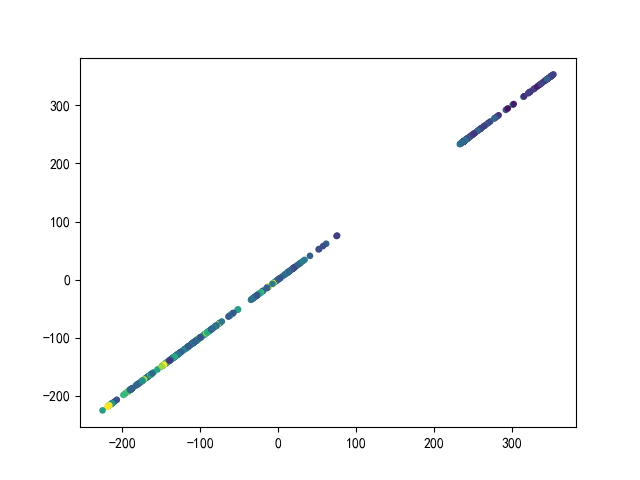
\includegraphics[width=0.3\linewidth]{img/pca-1.png}
	}
	\subfigure[主成分为2]{
		\label{fig::k2}
		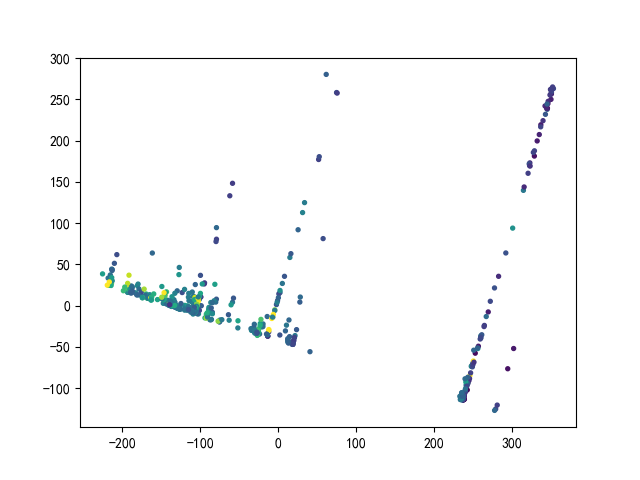
\includegraphics[width=0.3\linewidth]{img/pca-2.png}
	}
	\subfigure[主成分为3]{
		\label{fig::k3}
		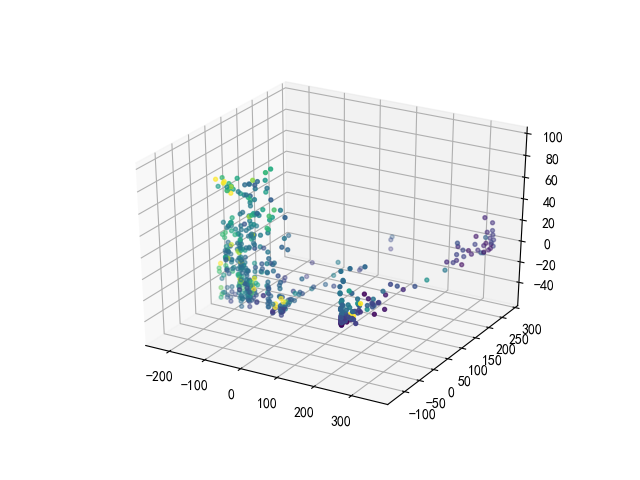
\includegraphics[width=0.3\linewidth]{img/pca-3.png}
	}
	\caption{PCA效果可视化(图中不同点的颜色代表不同的回归目标,即房价,颜色越接近则表示数值越接近)}
	\label{fig::single_salary}
\end{figure}


\begin{table}[H]
	\renewcommand\arraystretch{1.35}
	\caption{Boston数据集PCA降维效果比较}
	\label{tab:pca_res_com}
	\centering
	
	\begin{tabular}{c|c}
		\centering
		主成分个数 &   主成分方差占比之和 \\
		\hline
		1 & 0.80581 \\
		2 & 0.96887 \\
		3 & 0.99021 \\
		4 & 0.99717 \\
		5 & 0.99848 \\
		6 & 0.99921 \\
		7 & 0.99963 \\
		8 & 0.99988 \\
		9 & 0.99996 \\
		10 & 0.99999 \\
		11 & 0.99999 \\
		12 & 0.99999 \\
		13 & 1.00000 \\
	\end{tabular}
\end{table}

\begin{figure}[H]
	\centering
	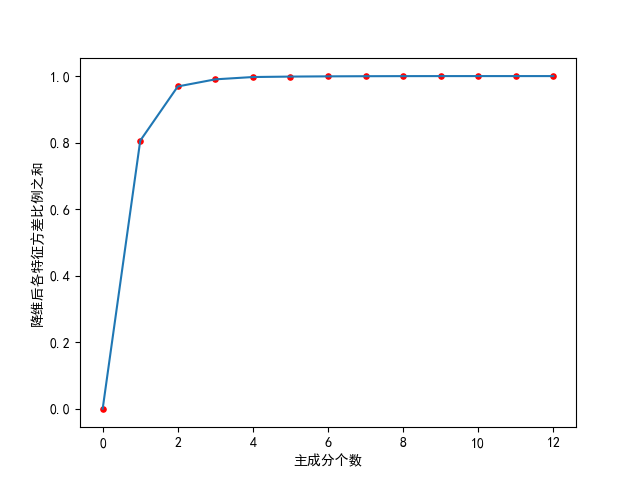
\includegraphics[width=0.73\linewidth]{img/kline.png}
	\caption{PCA对于Boston数据集的降维效果}
	\label{fig::kline}
\end{figure}


\newpage
\begin{appendix}
	\section{附录}
	\subsection{Boston数据集特征信息}
	\label{apd:boston_char}
	\begin{table}[H]
		\renewcommand\arraystretch{1.35}
		\caption{Boston数据集特征信息}
		\label{tab:boston_char}
		\centering
		
		\begin{tabular}{c|c|c}
			\centering
			编号 & 特征名 & 特征含义 \\
			\hline
			1 & CRIM & 城镇人均犯罪率 \\
			2 & ZN & 住宅用地超过 25000 sq.ft. 的比例 \\
			3 & INDUS & 城镇非零售商用土地的比例 \\
			4 & CHAS & 查理斯河空变量(如果边界是河流,则为1;否则为0) \\
			5 & NOX & 一氧化氮浓度 \\
			6 & RM & 住宅平均房间数 \\
			7 & AGE & 1940 年之前建成的自用房屋比例 \\
			8 & DIS & 到波士顿五个中心区域的加权距离 \\
			9 & RAD & 辐射性公路的接近指数 \\
			10 & TAX & 每 10000 美元的全值财产税率 \\
			11 & PTRATIO & 城镇师生比例 \\
			12 & B & 1000(Bk-0.63)\^ 2,其中 Bk 指代城镇中黑人的比例 \\
			13 & LSTAT & 人口中地位低下者的比例 \\			
		\end{tabular}
	\end{table}
	
	\subsection{主要代码}
	\label{apd:code}
	
\end{appendix}

%========================================================================
\end{document}